\section{Einführung}
\label{sec:intor}

Die vorliegende Aufgabe dreht sich um die Systemidentifikation zweier System.
Dafür wurden in der Aufgabenstellung jeweils ein FIR und ein IIR Filter gegeben.
Mit Hilfe der in der Vorlesung besprochenen adaptiven Filter sollte die Koeffizienten der gegebenen System identifiziert werden.
Als Vorbereitung auf die Systemidentifikation wurden der Least-Mean-Square Algorithmus (LMS) und der Recursive-Least-Squares Algorithmus mit Vergessenfaktor (RLS) implementiert.
Die Implementation erfolgte in Python \footnote{Software Repository:\url{https://github.com/Foaly/AdaptiveFilter}} anhand der Rechenvorschrift nach Moschytz \cite{moschytz2000book} (LMS nach S. 85 und RLS nach S.145).

\section{FIR-Filter}
\label{sec:fir}

Die erste Aufgabe ist die Systemidentifikation eines FIR Filters mit 5 Koeffizienten.
Das System wird mit Hilfe des LMS und KLS (mit Vergessensfaktor) Algorithmus identifiziert.
Der Einfluss unterschiedlicher Parameter, wie die Anzahl der Filterkoeffizienten, die Varianz des hinzugefügten Rauschens und die Werte für Schrittweite oder Vergessensfaktor auf das Ergebnis wird dabei untersucht.

In den entstandenen Plots wird der quadratischen Fehlers (Mean-Square-Error bzw. MSE) über den zeitlichen Verlauf in Samplen dargestellt. 
Ein gegen 0 konvergierender Verlauf des Fehlers ist wünschenswert, da dies bedeutet, dass die Differenz zwischen Ausgang des Filters und dem gewünschten Signal kleiner wird und der damit Algorithmus sich selbst verbessert.
Die gestrichelte Rote Linie zeigt den Durchschnittswert des Fehlers an, welche es vereinfacht den Wert abzulesen, auf den der Fehler konvergiert.
Außerdem sei angemerkt, dass der Plot des Fehler mit einem Rolling Average von 30 Samplen geglättet wurde, um einzelne Ausreißer zu entfernen und die Lesbarkeit zu erhöhen.

\subsection{Anzahl an Filterkoeffizienten}

Die Anzahl der Filterkoeffizienten ist einer der Parameter, der die Systemidentifikation am Stärksten beeinflusst. 
Zu erwarten wäre, dass sich das zu identifizierende System mit weniger Koeffizienten als nötig nicht hinreichend genau abbilden lässt. 
Nach dem Testen verschiedener Mengen an Filterkoeffizienten ($N \in \{1, 2, 5\}$) erwies sich diese Annahme auch als korrekt.
Dabei fällt auf, dass dem LMS Algorithmus die Approximation mit zu wenig Filterkoeffizienten wesentlich besser gelingt, als der RLS Algorithmus (vgl. die beiden Plots in \ref{fig:N1} und \ref{fig:N2}).

\begin{figure}[H]
  \centering
      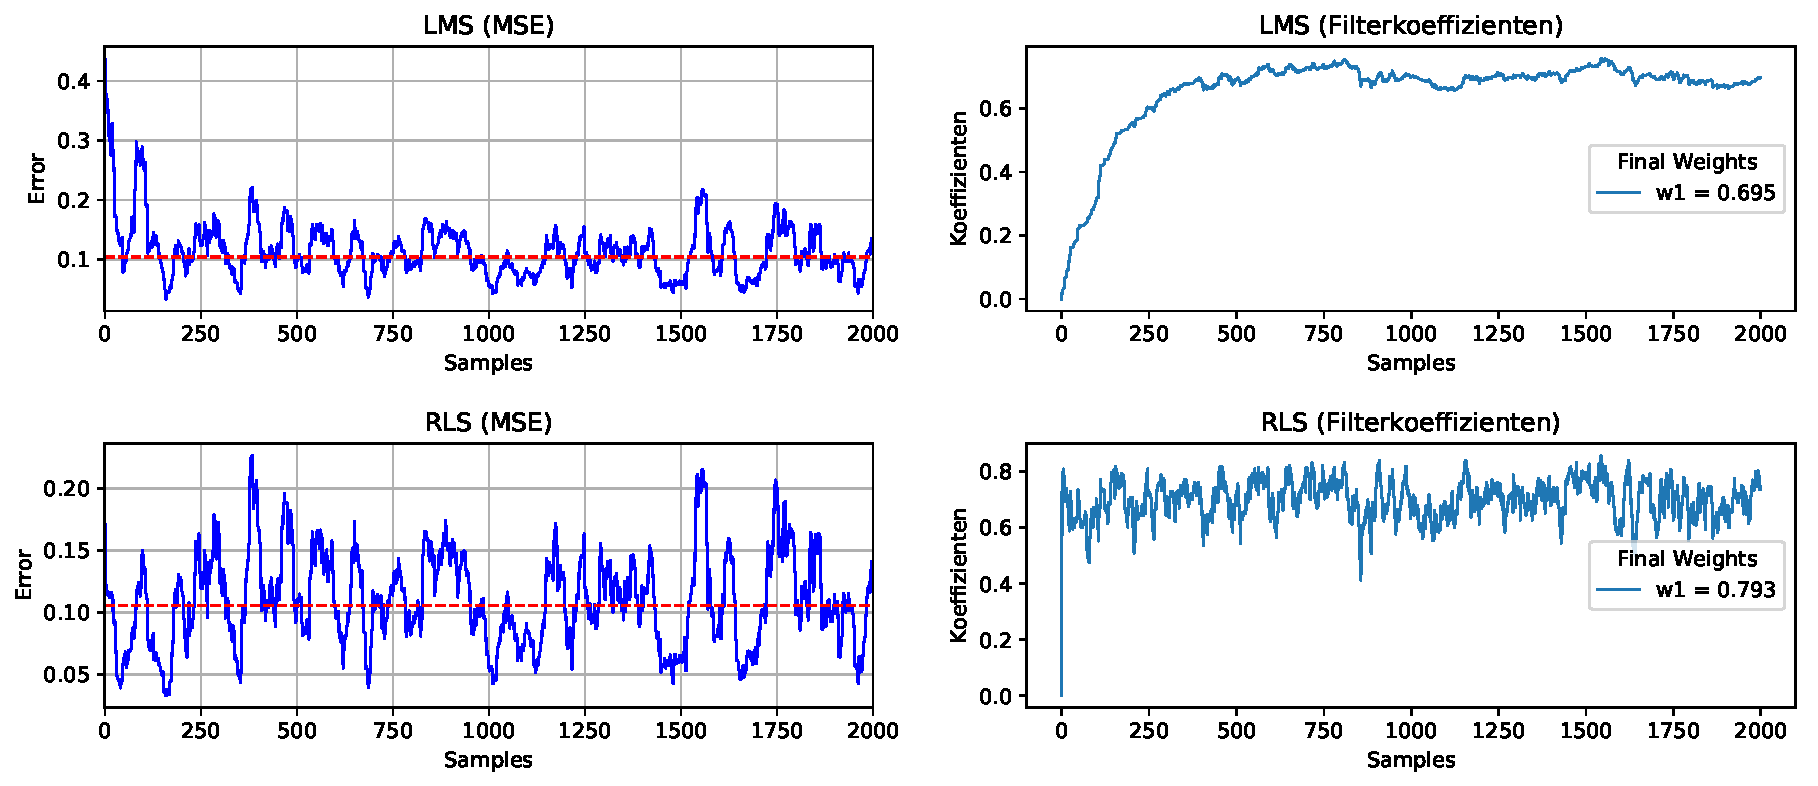
\includegraphics[width=0.6\textwidth]{{{figures/N_1_var_0.001}}}
 \caption{Vergleich zwischen LMS und RLS mit je einem Filterkoeffizienten (N=1)}
	\label{fig:N1}
\end{figure}

\begin{figure}[H]
  \centering
      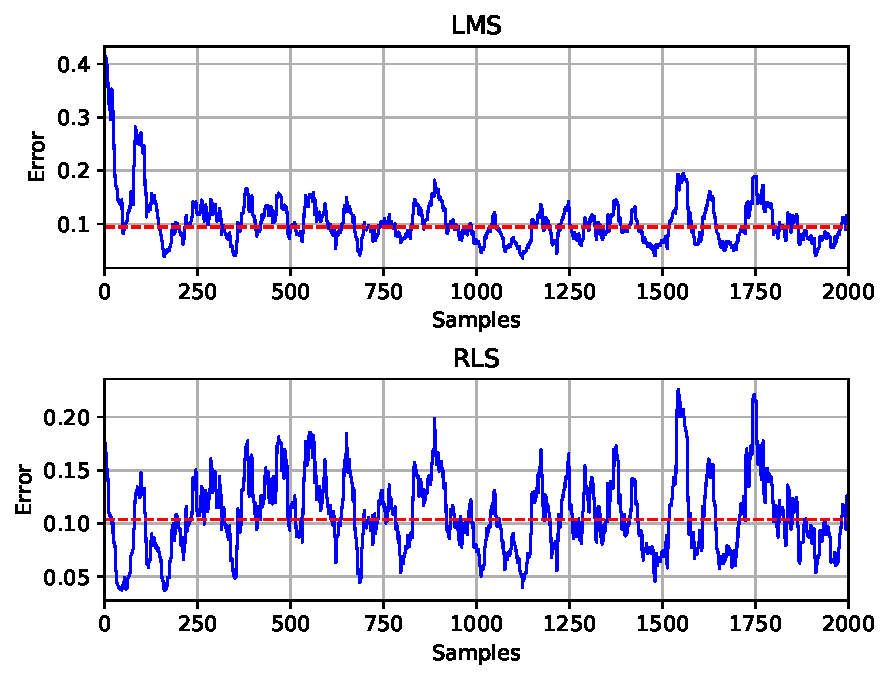
\includegraphics[width=0.6\textwidth]{{{figures/N_2_var_0.001}}}
 \caption{Vergleich zwischen LMS und RLS mit je zwei Filterkoeffizienten (N=2)}
	\label{fig:N2}
\end{figure}

\begin{figure}[H]
  \centering
      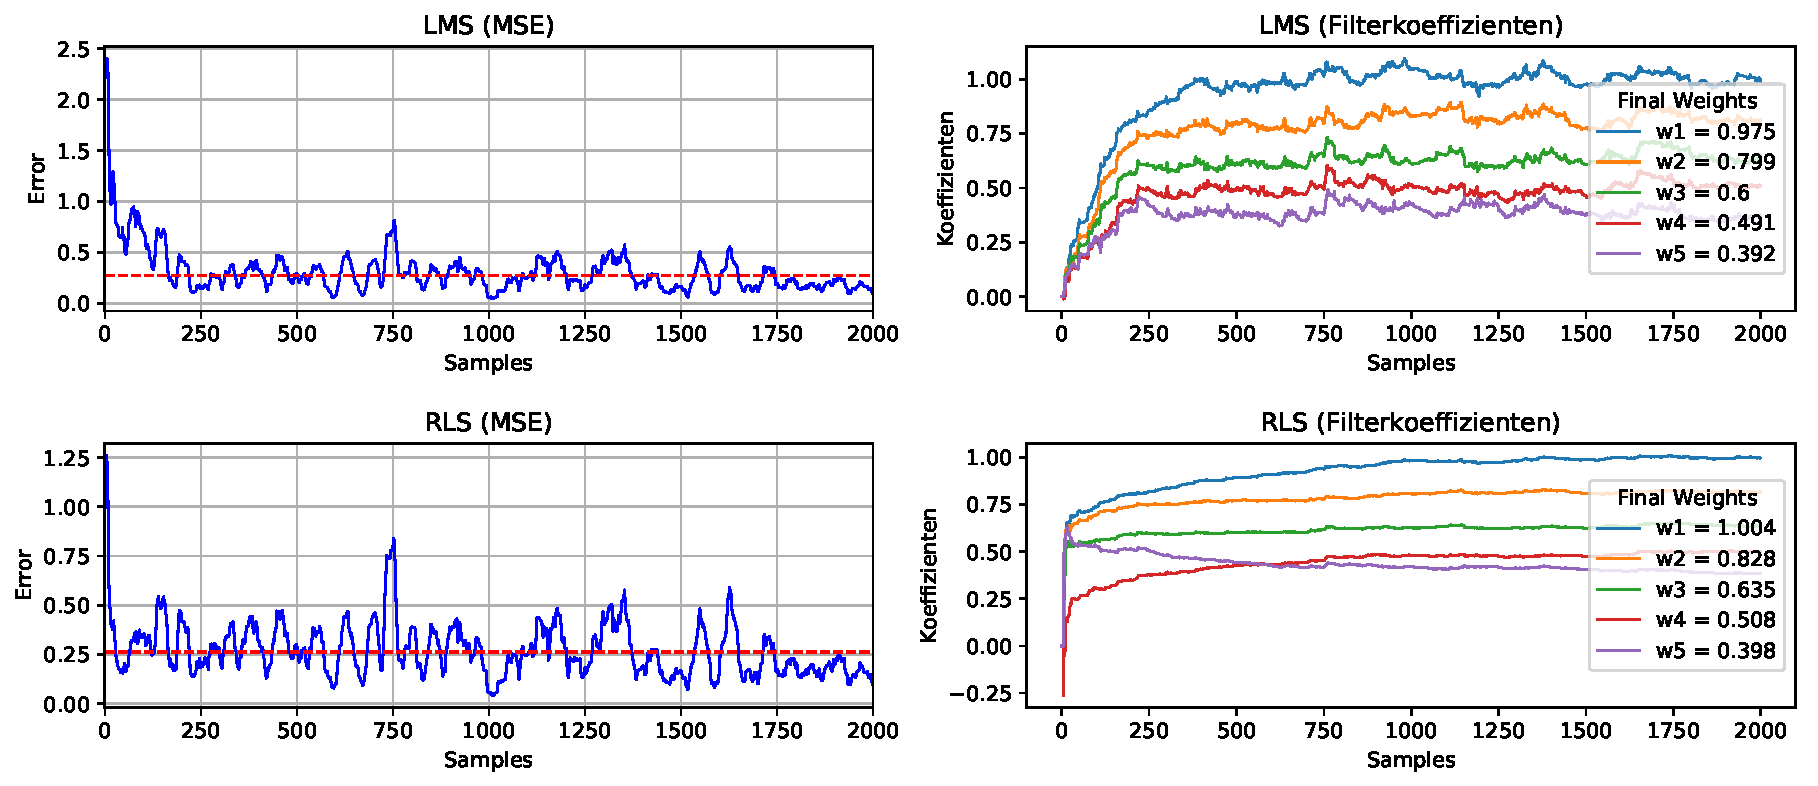
\includegraphics[width=0.6\textwidth]{{{figures/N_5_var_0.001}}}
 \caption{Vergleich zwischen LMS und RLS mit je fünf Filterkoeffizienten (N=5)}
	\label{fig:N5}
\end{figure}

\subsection{Einfluss der Rauschvarianz}
In der Messstrecke des Systems wird ein AWGN (Additive White Gaussian Noise bzw. Additives Weißes Gausverteiltes Rauschen) hinzugefügt.
Dies ist als $n[k]$ in der schematischen Darstellung A.2 in \cite{moschytz2000book} (S. 211) der Messstrecke gekennzeichnet. 
Dadurch lässt sich Testen, welche Algorithmus stabiler und weniger anfällig gegenüber Rauschen ist und sich besser für eine schlechte Übertragungsstrecke einsetzen lässt.
Für die Varianz des Rauschens $\sigma^2$ wurden verschiedene Werte angenommen ($\sigma^2 \in \{0.001, 0.1, 1, 10\}$) und ihr Einfluss auf das Fehlerverhalten der adaptiven Algorithmen untersucht.
Wenig überraschend bedeutet eine Zunahme der Varianz des Rauschen ebenfalls eine Zunahme im quadratischen Fehler.
Vergleicht man die Abbildung \ref{fig:N5,} welches mit einem AWGN mit $\sigma^2 = 0.001$ berechnet wurde, mit der Abbildung \ref{fig:sig0.1} ($\sigma^2 = 0.1$) so wird deutlich wie stark das Rauschen die Leistung des adaptiven Filters schwächt.
In Abbildung \ref{fig:N5}, \ref{fig:sig0.1} und \ref{fig:sig1} ist noch erkennbar, dass die Filter mit ansteigenden Werten für $\sigma^2$ auf einen jeweils angestiegenen Fehlerwert konvergieren.
In \ref{fig:sig10} mit $\sigma^2 = 10$ ist kein Konvergieren mehr sichtbar.
Bei Betrachten der Plots mit verschiedenen Werten für $\sigma^2$ fällt erneut auf, dass der LMS im Vergleich zum RLS eine stärke Toleranz gegenüber Rauscheinflüssen aufweist.
Ebenfalls auffällig ist die deutliche Ähnlichkeit der beiden Kurven der unterschiedlichen Algorithmen in Abbildung \ref{fig:sig10}.
Dies lässt darauf schließen, dass der Signal-Rausch-Abstand (SNR) so gering ist, dass das Rauschen das eigentlich Signal nahezu komplett überdeckt.

\begin{figure}[H]
  \centering
      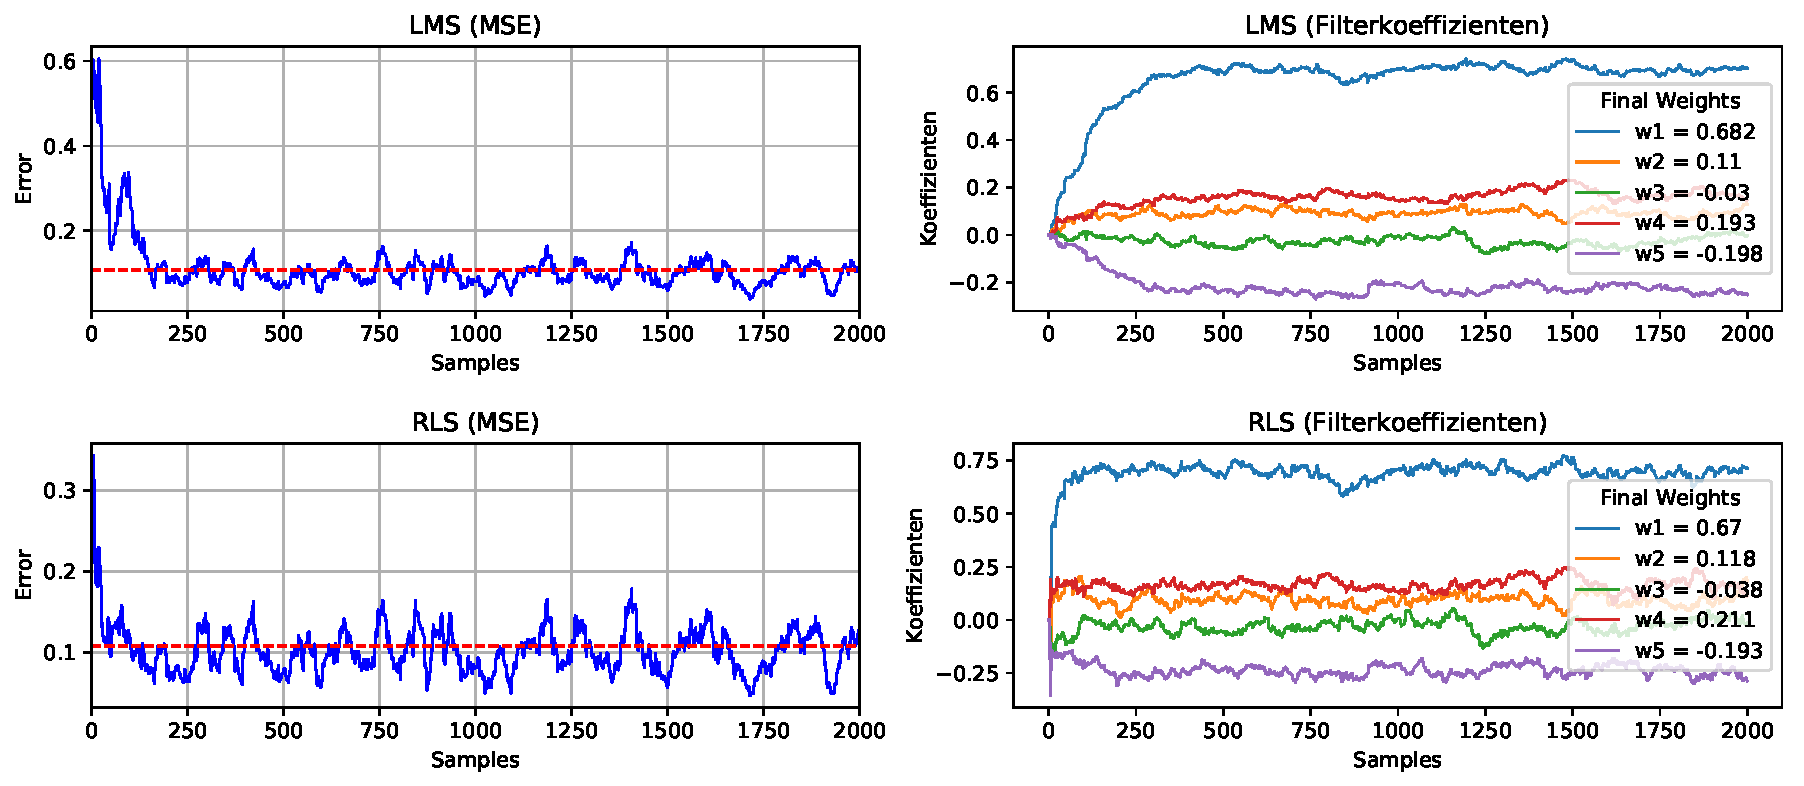
\includegraphics[width=0.6\textwidth]{{{figures/N_5_var_0.1}}}
 \caption{Vergleich zwischen LMS und RLS bei einem AWGN von $\sigma^2 = 0.1$  (N=5)}
	\label{fig:sig0.1}
\end{figure}

\begin{figure}[H]
  \centering
      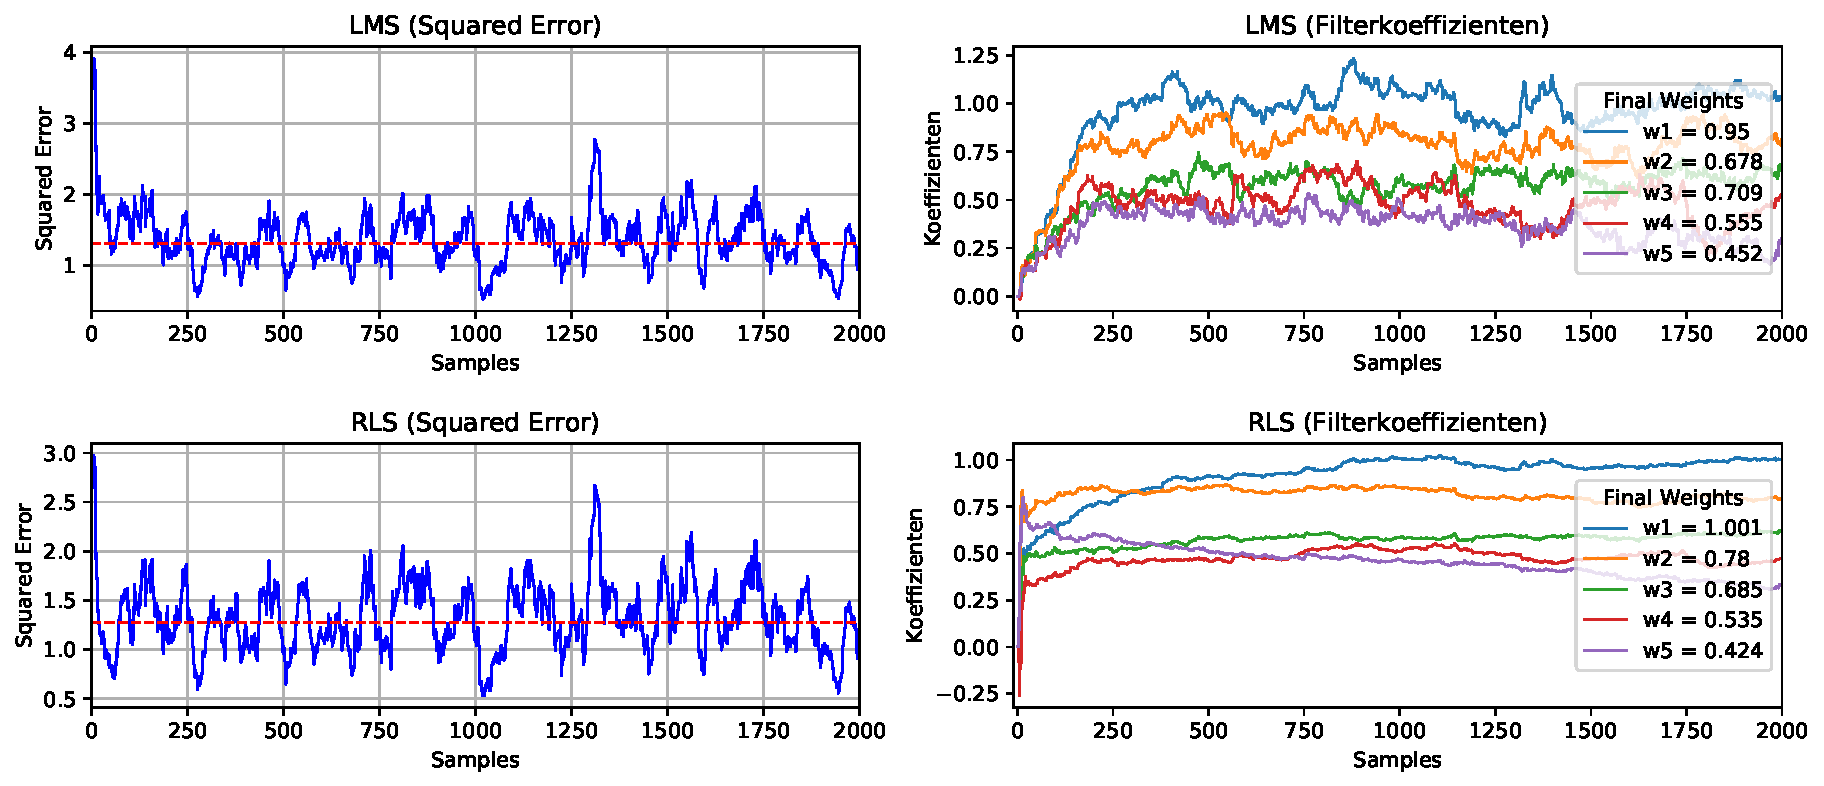
\includegraphics[width=0.6\textwidth]{{{figures/N_5_var_1.0}}}
 \caption{Vergleich zwischen LMS und RLS bei einem AWGN von $\sigma^2 = 1$  (N=5)}
	\label{fig:sig1}
\end{figure}

\begin{figure}[H]
  \centering
      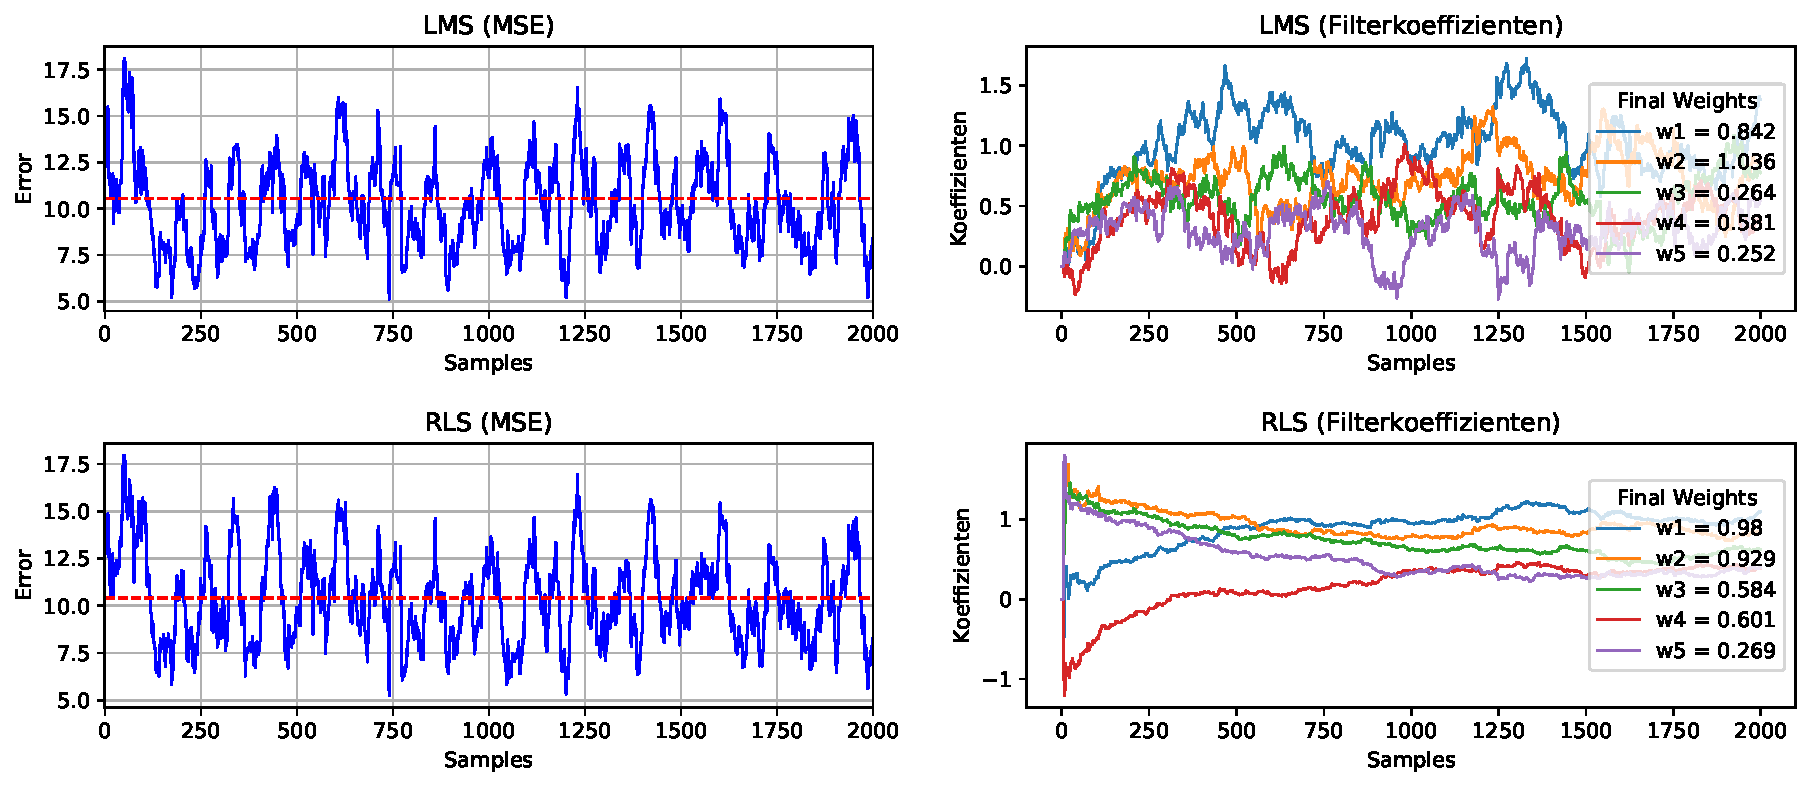
\includegraphics[width=0.6\textwidth]{{{figures/N_5_var_10.0}}}
 \caption{Vergleich zwischen LMS und RLS bei einem AWGN von $\sigma^2 = 10$  (N=5)}
	\label{fig:sig10}
\end{figure}


\subsection{Einfluss des Vergessensfaktors $\rho$}

Bisher bei allen Plots 0.9

\subsection{Einfluss des Schrittweite $\mu$}

Bisher bei allen Plots 0.01



\subsection{Wahl des Lernalgorithmus}
\files{main.py}


\section{IIR-Filter}
\label{sec:iir}

\subsection{Anzahl an Filterkoeffizienten}
\subsection{Wahl des Lernalgorithmus}
\subsection{Einfluss der Varianz}


\section{Systemwechsel}
\label{sec:3}

\subsection{Adaptionsverhalten}


\section{Kernel Least Mean Squares}
\label{sec:4}


\section{Fehlerfunktion(en)}
